\chapter{Aktorenmodell}

In diesem Kapitel wird mit Aktoren ein Modell für nebenläufige Programmierung vorgestellt, das ausschließlich auf dem Austausch von asynchronen Nachrichten basiert. Dieses Modell eignet sich vor allem für Systeme, in denen es eine große Anzahl von gleichzeitigen Aufgaben gibt. Zu diesen Szenarien zählen Systeme mit vielen Benutzern, gleichermaßen wie dem Internet der Dinge, das viele  Geräte miteinander vernetzt.

Am Beginn dieses Kapitels werden die theoretischen Grundlagen des Aktorenmodells erläutert. Anschließend wird mit der Sprache Erlang eine der ersten populären Implementierungen des Aktorenmodells präsentiert. Darauf aufbauend wird mit dem virtuellen Aktorenmodell eine mögliche Vereinfachung des Programmiermodells vorgestellt und diskutiert. Zum Abschluss dieses Kapitels wird noch die Beziehung des Aktorenmodells zur Microservice"=Architektur und anderen Technologien analysiert.

\section{Grundlagen des Aktorenmodells}
\label{sec:actor-model}

Die ersten theoretischen Überlegungen über das Aktorenmodells stellten \citeauthor{Hewitt:1973:UMA:1624775.1624804} bereits 1973 in \cite{Hewitt:1973:UMA:1624775.1624804} an. Hewitt beschreibt einen Aktor als fundamentale Recheneinheit, mit der Fähigkeit  \textit{Berechnungen} durchzuführen, Daten zu \textit{speichern} und mit anderen Aktoren zu \textit{kommunizieren}. Diese allgemeine Definition wird durch folgende drei Axiome ergänzt, die ein Aktor erfüllen muss:

\begin{itemize}
	\item Ein Aktor kann neue Aktoren erzeugen,
	\item Nachrichten an andere Aktoren oder sich selbst senden und
	\item sein Verhalten ändern.
\end{itemize}

\noindent
Das Aktorenmodell ist nicht mit einem konkreten Programmierparadigma verbunden, sondern ein abstraktes Modell. Anschließend an diesen Abschnitt wird mit Erlang eine rein funktionale Implementierung vorgestellt und danach mit Project Orleans eine objektorientierte. Im Aktorenmodell finden sich viele Ideen aus der objektorientierten Programmierung, wie \zB Datenkapselung oder Nachrichtenaustausch wieder. Daher finden sich Entwickler mit einem Hintergrund in objektorientierter Programmierung oft sehr schnell mit der Funktionsweise des Aktorenmodells zurecht.

Ein einzelner Aktor hat nur begrenzte Möglichkeiten, daher kommen sie immer in ganzen Aktorsystemen vor. Da Aktoren eine sehr leichtgewichtige Einheit darstellen, können sehr viele Aktoren gleichzeitig in einem System existieren. Außerdem sind das Erzeugen und Zerstören von Aktoren sehr effiziente Operationen. Aktoren bilden zur Laufzeit ein dynamisches Netzwerk, oder um es in der Sprache der Graphentheorie auszudrücken, einen gerichteten Graphen.

In sequentiellen Programmen wird Nebenläufigkeit meistens dadurch erreicht, dass mehrere Ausführungsstränge auf die selben Daten -- also den selben Speicherbereich -- zugreifen. Natürlich muss der Zugriff auf diese Daten geschützt und koordiniert werden, was diese Art der Programmierung schwierig und fehleranfällig macht. Nebenläufigkeit durch Aktoren, oder im Allgemeinen durch Nachrichtenaustausch kann eine gute Alternative dazu sein. Aktoren besitzen keinerlei geteilten Speicher. Jede Information die sie benötigen, müssen sie für sich selbst lokal speichern, oder als Teil einer Nachricht gesendet bekommen. Der Zustand eines Aktors ist somit für die Umwelt und damit auch für andere Aktoren nicht sichtbar.

Die Verarbeitung der empfangenen Nachrichten führt jeder Aktor sequentiell durch. Aber alle Aktoren können diesen Vorgang parallel durchführen. Gesamtheitlich gesehen ist dieses Modell also inhärent nebenläufig und somit gut skalierbar, auch wenn jeder Aktor für sich sequentiell ist. Je mehr Rechenkerne oder sogar Rechner zur Verfügung stehen, desto mehr Aktoren können gleichzeitig arbeiten.

Der Nachrichtenaustausch zwischen Aktoren erfolgt asynchron. Sender und Empfänger sind somit voneinander zeitlich entkoppelt.  Eigentlich ist nur das Senden von Nachrichten asynchron, das Empfangen jedoch ist für den Aktor eine synchrone \bzw blockierende Operation. Synchrone Kommunikation kann aber über Bestätigungsnachrichten nachgebildet werden. Bis zur tatsächlichen Verarbeitung einer Nachricht wird sie in einer Warteschlange zwischengespeichert. Manche Implementierungen des Aktorenmodells, darunter auch Erlang, unterstützen ein selektives Empfangen. Das bedeutet, dass nur bestimmte Nachrichten verarbeitet werden und andere in dieser Zeit in der Warteschlange verbleiben.

Das Aktorenmodell macht keine Annahmen darüber, ob es auf einem einzigen oder auf einen verteilten System angewendet wird. Daher sind Programme die nach diesem Modell entwickelt wurden, ohne größere Änderung auf ein verteiltes System erweitert werden. Aktoren werden ohnehin nur über ihre Adressen angesprochen, die auch über Rechnergrenzen hinweg gültig haben. Sie benötigen auch keinen gemeinsamen Speicherbereich, der in einem verteilten System ohnehin nicht existiert.

Obwohl Programme im Stile des Aktorenmodells in vielen Fällen einfacher sind als Systeme mit geteilten Speicher, schützt es dennoch nicht vor allen Herausforderungen der parallelen Programmierung. Deadlocks, kritische Wettlaufsituation oder ähnliche Probleme können durch falsche Anwendung dennoch entstehen. Aber später in diesem Kapitel noch genauer erläuterte Mechanismen, wie Supervisorbäume und die Überwachung von Zeitüberschreitungen zeigen, wie man diese Probleme mindern kann.

\section{Erlang}
\label{sec:erlang}

Mit dem Ziel die Implementierung von hoch verfügbaren und verteilten Telekommunikationsanwendungen zu erleichtern, begann \citeauthor{Armstrong:1997:DE:258948.258967} 1985 die  Programmiersprache Erlang zu entwickeln~\cite{Armstrong:1997:DE:258948.258967}. In den Fokus seiner Bemühungen stellte er die Vereinfachung von nebenläufiger Programmierung. Die Begründung dahinter liegt darin, dass auch die reale Welt, die mit Software nachgebildet wird, inhärent nebenläufig ist. In jedem Augenblick passieren eine Unmenge an gleichzeitigen Ereignissen, die wir asynchron verarbeiten. Sequentielle Abläufe sind hier eher die Ausnahme. Trotzdem versuchen viele Programmiersprachen diese Tatsache zu ignorieren und stellen die sequentielle Hintereinanderausführung von Aktivitäten in den Vordergrund.

Um die Rolle der Nebenläufigkeit zu unterstreichen und Erlang von anderen Sprachen zu unterscheiden, bezeichnet Armstrong in \cite[19]{armstrong03} den Stil von Erlang als \textit{nebenläufigkeitsorientierte Programmierung}. Weitere wesentliche Einflussfaktoren auf die Sprache sind die funktionale und teilweise die logische Programmierung, in Anlehnung an die Sprache Prolog.

Obwohl Erlang und das Aktorenmodell ein wenig in Vergessenheit geraten sind, erleben beide derzeit wieder einen neuen Aufschwung. Das Interesse verzeichnete einen steilen Anstieg, nachdem die Kommunikationsplattform WhatsApp bekanntgab, dass sie mit ihrem in Erlang entwickelten Plattform bis zu siebzig Millionen Nachrichten pro Sekunde verarbeiten~\cite{ErlangWhatsApp}.

\subsection{Einführung in die Sprache Erlang}

Dieser Abschnitt beinhaltet eine Einführung in die Syntax und Konzepte von Erlang, damit auch Leser ohne Vorkenntnisse in Erlang den Beispielen in diesem Kapitel folgen können. Die Sprache Erlang an sich ist wegen des minimalistischen Typsystems und der geringen Anzahl an Sprachfunktionen sehr einfach. Umfassendere Einführungen in Erlang geben die offizielle Dokumentation, \cite{Hebert:2013:LYE:2543986} und \cite{armstrong03}, auf denen auch ein wesentlicher Teil dieses Kapitels basiert.

\subsubsection{Typsystem}
\label{subsubsec:erlang-typesystem}

Die Sprache Erlang lässt sich als dynamisch und stark typisiert charakterisieren. Das sehr einfache Typsystem umfasst acht primitive und mit Tupel \bzw Listen zwei zusammengesetzte Datentypen, die nachfolgend noch erläutert werden.

In \cite{Marlow:1997:PSS:258948.258962} wurde versucht, Erlang um ein statisches Typsystem zu erweitern, um Programmierfehler schon zur Übersetzungszeit zu identifizieren. Obwohl dieser Ansatz teilweise erfolgreich war, wurde er nicht weiter verfolgt, weil nicht alle Teile der Sprache typisiert werden konnten~\cite[14]{Armstrong:2007:HE:1238844.1238850}. Später wurde ein Werkzeug für leichtgewichtige statische Code"=Analyse mit dem Namen \textit{Dialyzer} entwickelt~\cite{ErlangWarStory}. Im Gegensatz zu dem in \cite{Marlow:1997:PSS:258948.258962} verfolgten Ansatz, benötigt der Dializer keine zusätzlichen Typ"=Annotationen durch den Programmierer und erkennt dennoch die meisten Fehler, die auch ein statisches Typsystem erkennen könnte.

\subsubsection{Variablen}

Wie in vielen funktionalen Sprachen sind Variablen unveränderbar. \Dah es kann nur einmal ein Wert zugewiesen werden. In Erlang spricht man häufiger vom "`Binden"' einer Variable an einen Wert. Per Konvention beginnen alle Variablennamen mit einem Großbuchstaben. Programm~\ref{prog:erlang-vars} zeigt einige Beispiele für die Verwendung von Variablen.

\begin{program}[!hbt]
\caption{Verwendung von Variablen in Erlang}
\label{prog:erlang-vars}
\begin{ErlangCode}
Var1 = 1 + 2.
Var1 = Var1. % succeeds because left and right hand side are equal
Var2 = Var1 + 1. % succeeds and Var2 = 4.
Var1 = Var1 + 1. % fails because left and right hand side don't unify
\end{ErlangCode}
\end{program}

\subsubsection{Atome}

Atome bezeichnen in Erlang einen primitiven Datentyp, der wie ein Literal oder eine Konstante zu verstehen ist. Während Variablennamen immer mit einem Großbuchstaben beginnen, müssen Atome mit einem Kleinbuchstaben beginnen, damit sie unterscheidbar sind. In Programm~\ref{prog:erlang-atom} ist die Zuweisung eines Atoms an eine Variable gezeigt.

\begin{program}[!hbt]
\caption{Verwendung eines Atoms in Erlang}
\label{prog:erlang-atom}
\begin{ErlangCode}
Var3 = myatom.
\end{ErlangCode}
\end{program}

\subsubsection{Tupel und Listen}

Ein Tupel ist eine endliche Folge fixer Größe, die mehrere Elemente zu einem Verbund zusammenfasst. Die Anzahl der Elemente in einem Tupel ist endlich und nicht veränderbar. Neben Tupel besitzt Erlang auch einen Datentyp für Listen, der eine beliebige Anzahl von Elementen aufnehmen kann. Im Gegensatz zu anderen Programmiersprachen müssen die Typen der Listenelemente nicht homogen sein. Tupel und Listen scheinen äußerlich sehr ähnliche Fähigkeiten zu haben. Generell gilt aber, dass Tupel für Datenstrukturen und Listen für Sequenzen von Elementen vorgesehen sind. Einige Beispiele für die Deklaration von Listen sind in Programm~\ref{prog:erlang-lists} angeführt.

\begin{program}[!hbt]
\caption{Verwendung von Listen in Erlang}
\label{prog:erlang-lists}
\begin{ErlangCode}
Person1 = { alice, "Fake Street 42", 1234 }.
Person2 = { bob, "Main Avenue 1", 5678 }.
Person3 = { person, alice, "Fake Street 42", 1234 }. % mimics a class
List1 = [ 1, two, "three" ].
List2 = [ 1 | [2 | [ 3 | [] ] ] ].
List3 = [ Person1, Person2 ].
\end{ErlangCode}
\end{program}

\subsubsection{Module und Funktionen}

Module sind Dateien, die mehrere logisch zusammengehörende Funktionen zu einer Einheit gruppieren. Das ermöglicht eine bessere Organisation des Quelltexts eines Programms und hilft, Namenskonflikte aufzulösen. Nur explizit exportierte Funktionen sind von außerhalb aufrufbar. Ansonsten sind Funktion nur innerhalb ihres eigenen Moduls sichtbar.

Eine Funktion besteht aus mehreren Funktionsanweisungen, die wiederum aus mehreren Ausdrücken bestehen können. Der Kopf einer Funktionsanweisung definiert ein Muster, das bei der Aktivierung einer Funktion mit den tatsächlichen Funktionsparametern verglichen wird. Diejenige Funktionsanweisung, deren Muster als erstes mit den Funktionsparametern übereinstimmt, wird schlussendlich ausgeführt. In funktionalen Sprachen, somit auch in Erlang, wird ein Mustervergleich -- \textit{engl. Pattern Matching} -- oft für Fallunterscheidungen verwendet. Erlang unterstützt noch weitere Formen von Mustervergleichen, von denen einige im Laufe dieses Kapitels noch verwendet werden. In Programm~\ref{prog:erlang-module} ist die Deklaration eines Moduls und einer Funktion gezeigt. Die Funktion \lstinline{area} besteht aus vier Funktionsanweisungen mit unterschiedlichen Mustern im Kopf der Anweisung.

\begin{program}[!hbt]
\caption{Deklaration eines Moduls in Erlang}
\label{prog:erlang-module}
\begin{ErlangCode}
-module(shape).
-export([area/1]).
area({square, Width}) -> Width * Width;
area({rectangle, Width, Height}) -> Width * Height;
area({circle, Radius}) -> math:pi() * Radius * Radius;
area(_) -> erlang:error(unknown_shape).
\end{ErlangCode}
\end{program}

\subsection{Prozesse}
\label{subsec:erlang-processes}

Einer der zentralen Bestandteile von Erlang sind Prozesse. Dabei handelt es sich nicht um Betriebssystemprozesse, sondern leichtgewichtige Prozesse in der Erlang"=Laufzeitumgebung. Die Laufzeitumgebung ist eine abstrakte virtuelle Maschine, die viele Aufgaben eines Betriebssystem imitiert. Dazu zählen das Prozess"=Scheduling, der Nachrichtenaustausch, automatische Speicherbereinigung \usw

Die Funktion \lstinline{spawn} startet einen neuen Prozess. Dabei muss als Argument eine Lambda"=Funktion, oder der Funktions"= und Modulname der auszuführenden Funktion übergeben werden. Nachdem ein Prozess gestartet wurde, kann er Nachrichten von anderen Prozessen empfangen. Der Nachrichtenaustausch zwischen Prozessen erfolgt asynchron. Jeder Prozess besitzt eine eigene Warteschlange, in der Nachrichten bis zur eigentlichen Verarbeitung zwischengespeichert werden.

Es gibt in Erlang keinen gemeinsamen Speicher, auf den mehrere Prozesse zugreifen können. Benötigt ein Prozess Informationen eines anderen Prozesses, muss er diese als Nachricht gesendet bekommen. Daraus ergibt sich ein sehr sauberes Programmiermodell, in dem ganz genau klar ist, wer die Verantwortung für die Speicherung bestimmter Daten hat und wie der Datenfluss aussieht. Im Gegensatz dazu ist es bei geteilten Daten, die von mehreren Stellen verändert werden, immer schwierig nachzuvollziehen, wie eine Änderung zustande kam.

Das Senden einer Nachricht schlägt niemals fehl, selbst wenn der Empfänger nicht existiert. Ein synchroner Nachrichtenaustausch kann nur mit Hilfe von Bestätigungsnachrichten nachgebildet werden. Dabei ist es aber wichtig, adäquate Zeitbeschränkungen zu verwenden, sodass Fehler, wie \zB ein abgestürzter Empfänger, erkannt werden können.

In Programm~\ref{prog:erlang-processes} sind einige wichtige Konstrukte im Zusammenhang mit Erlang"=Prozessen demonstriert. Die linke Spalte zeigt die Implementierung eines einfachen Prozesses der Grundrechenoperationen durchführen und Zwischenergebnisse auf dem Bildschirm ausgeben kann. In der linken Spalte in den Zeilen acht bis dreizehn sind Mustervergleiche mit den empfangenen Nachrichten definiert. Je nach Nachricht wird eine andere Aktion ausgeführt. Der Zustand des Prozesses -- die Zwischensumme -- ist ein Parameter der Funktion \lstinline{loop}. Nach diesem oder einem ähnlichen Schema sind im Prinzip alle Prozesse in Erlang gestaltet. Da ein Prozess keine globalen Daten verändern kann, muss er seinen Zustand immer als Parameter in den nächsten Rekursionsschritt mitnehmen. Der Prozess in Programm~\ref{prog:erlang-processes} kann durch das Senden des Atoms \lstinline{stop} sauber beendet werden, da dieser Zweig der Nachrichtenbearbeitung keinen weiteren Rekursionsschritt mehr durchführt.

\begin{program}[!hbt]
\caption{Kommunikation zwischen Prozessen in Erlang}
\label{prog:erlang-processes}
\noindent\begin{minipage}[t]{.52\textwidth}
\lstset{showlines=true}
\begin{ErlangCode}
-module(calculator).
-export([init/0, loop/1]).

init() ->
  spawn(fun () -> loop(0) end).

loop(Total) ->
  receive
    { add,  X } -> loop(Total + X);
    { mult, X } -> loop(Total * X);
		{ divi, X } -> loop(Total / X);
    result      -> io:write(Total),
									 loop(Total);
    stop    		-> ok
  end.
\end{ErlangCode}

\end{minipage}\hfill
\begin{minipage}[t]{.44\textwidth}
\lstset{showlines=true}
\begin{ErlangCode}
% compile
c(calculator).
% start the process
Pid = calculator:init().
% send messages by process id
Pid ! { add, 6 }.
% register a name
register(calc_server, Pid).
% send messages by name
calc_server ! { mult, 7 }.
Pid ! result. % prints 42
calc_server ! stop.
% next message won't arrive,
% but no error is raised
calc_server ! result.
\end{ErlangCode}

\end{minipage}
\end{program}

Auf der rechten Seite in Programm~\ref{prog:erlang-processes} ist die Interaktion mit dem gerade erläuterten Prozess demonstriert. Der beschriebene Quelltext wird ebenfalls in einem Prozess ausgeführt, dessen Erzeugung aber nicht explizit dargestellt ist. In Zeile vier wird der Variable \lstinline{Pid} die eindeutige Prozess"=Identifikationsnummer des gestarteten Prozesses zugewiesen. Mit dieser Nummer können Nachrichten an den Prozess, sogar Rechnergrenzen übergreifend, adressiert werden. Wie Zeile sieben zeigt, kann auch ein Name für einen gestarteten Prozess vergeben werden. Mit dem Infix"=Operator \lstinline{!} werden Nachrichten, die jeden beliebigen Erlang"=Typ entsprechen können, an einen Prozess gesendet. Es ist jedoch zu beachten, dass eine vollständige Kopie der Nachricht versendet wird, weil möglicherweise die Nachricht  über das Netzwerk an einen entfernten Rechner zu transportieren ist.

\subsection{Open Telecom Platform}

Auch wenn Erlang die Entwicklung von hoch verfügbaren und skalierbaren Anwendungen wesentlich erleichtert, bleibt es dennoch mit den einfachen Möglichkeiten die Erlang bietet sehr zeitaufwändig und komplex. Aus diesem Grund wurden für viele immer wiederkehrende Aufgaben eine Bibliothek entwickelt, die allgemeine Probleme löst und dem Entwickler viel Arbeit abnimmt.  Weil diese Bibliothek ursprünglich für Telekommunikationsanwendungen gedacht war, trägt sie den Namen \textit{Open Telecom Platform (OTP)}. Abgesehen vom Namen hat die Funktionalität dieser Bibliothek aber nichts mit dem Telekommunikationsbereich gemein und ist für alle Arten von Anwendungen geeignet. Neben sehr vielen nützlichen Hilfsfunktionen, beinhaltet die OTP auch eine Menge Hilfswerkzeuge, wie \zB den Erlang"=Compiler oder das in \ref{subsubsec:erlang-typesystem} erwähnte Werkzeug für statische Code"=Analyse.

In den nachfolgenden Abschnitten werden mit Supervision und endlichen Automaten zwei wichtige Teilbereiche von Erlang erläutert. Für beide beinhaltet die OTP"=Bibliothek bereits generische Implementierungen. 

\subsection{Supervision}
\label{subsec:erlang-supervision}

Das Konzept der Supervision ist einer der Gründe, warum 
Erlang für besonders fehlertolerante Software bekannt ist. Ein weiterer Grund ist die Organisation der Programme in voneinander isolierte Prozesse, in denen jeder seine eigene Fehlerdomäne bildet. Wenn ein Prozess einen Fehler verursacht, sind andere Prozesse davon nicht direkt beeinflusst. Anstelle eines defensiven Programmierstils ist es in Erlang üblich, Prozesse einfach abstürzen zu lassen, wenn sie ihre Arbeit nicht ordnungsgemäß ausführen konnten~\cite[104]{armstrong03}. Es ist die Aufgabe eines anderen Prozesses zu entscheiden, wie mit einem Fehler umgegangen werden soll. Grundsätzlich werden Prozesse in zwei Kategorien eingeteilt, die immer paarweise auftreten:

\begin{itemize}
	\item \textit{Arbeiterprozesse} erledigen die eigentliche Arbeit und beinhalten kaum Fehlerbehandlungslogik.
	\item \textit{Supervisorprozesse} haben die Aufgabe, Arbeiterprozesse zu überwachen und im Fehlerfall darauf zu reagieren.
\end{itemize}

Mehrere Prozesse können zu einer Einheit verbunden werden, sodass ein Absturz eines Prozesses auch die anderen Prozesse beendet. Die Funktion \lstinline{link} erzeugt die beschriebene symmetrische Verbindung zwischen zwei Prozessen. Meistens wird aber die Funktion \lstinline{spawn_link} verwendet, die das Starten und Verbinden in einem atomaren Schritt durchführt. Ansonsten könnte es zu einer kritischen Wettlaufsituation kommen, in der ein Prozess terminiert, bevor er verbunden wurde.

Nach dem Beenden eines Prozesses wird eine spezielle Nachricht an alle verbundenen Prozesse gesendet, die sich daraufhin selbst beenden. Es gibt aber spezielle System"=Prozesse, die eine Terminierungsnachricht wie eine gewöhnliche Nachricht empfangen und verarbeiten können. Um einen Prozess zu einem System"=Prozess zu befördern, muss nur die Eigenschaft \lstinline{trap_exit} gesetzt werden. System"=Prozesse übernehmen üblicherweise die Aufgaben eines Supervisors, weil sie entscheiden können, was mit einem Arbeiterprozess der sich erwarteten oder unerwarteten beendet hat, geschehen soll.

In Programm~\ref{prog:erlang-supervision} wird der in Programm~\ref{prog:erlang-processes} implementierte Prozess um einen Supervisor erweitert. Immer wenn der Arbeiterprozess abstürzt, \zB bei einer Division durch Null, bekommt der Supervisor eine Terminierungsnachricht. Anschließend startet dieser den Arbeiterprozess neu. Diese extrem simplifizierte Fehlerbehandlungsstrategie ist für ein reelles Szenario selbstverständlich nicht ausreichend. Er versucht unendlich oft, den Prozess sofort neu zu starten. Außerdem kann dieser Supervisor nur einen einzigen Arbeiterprozess überwachen. Im Laufe dieses Abschnitts wird noch gezeigt, welche intelligenteren Strategien die OTP"=Bibliothek bietet.

\begin{program}[!hbt]
\caption{Prozessüberwachung in Erlang}
\label{prog:erlang-supervision}
\noindent\begin{minipage}[t]{.52\textwidth}
\lstset{showlines=true}
\begin{ErlangCode}
-module(sup).
-export([start/4, init/4]).

start(Name, M, F, A) ->
  spawn(?MODULE,init,[Name,M,F,A]).

init(Name, Mod, Fun, Args) ->
  process_flag(trap_exit, true),
  loop(Name, Mod, Fun, Args).

loop(N, M, F, A) ->
  register(N,Pid=spawn_link(M,F,A)),
  receive
    { 'EXIT', Pid, normal } -> ok;
    { 'EXIT', Pid, Reason } -> 
      loop(Name, M, F, A);
    { 'EXIT', From, _ } -> 
			exit(shutdown)
  end.
\end{ErlangCode}

\end{minipage}\hfill
\begin{minipage}[t]{.44\textwidth}
\lstset{showlines=true}
\begin{ErlangCode}
c(calculator), c(sup).
sup:start(
  calc_server, 
  calculator, loop, [0]
).

% find the id for a 
% registered name
whereis(calc_server).
% some id like <0.84.0>
calc_server ! {add, 1}.
calc_server ! { divi, 0 }.
% worker crashed

whereis(calc_server). 
% process was restarted and
% got a new id, but it can
% still addressed by name
calc_result ! result.
\end{ErlangCode}

\end{minipage}
\end{program}

Ein Verhalten -- \textit{engl. Behavior} -- in Erlang ist mit einer abstrakten Klasse in objektorientierten Sprachen vergleichbar. Es bietet eine gewisse Grundfunktionalität, die der Verwender aber noch spezialisieren muss. \Dah der Verwender implementiert die vom Verhalten vorgegeben Funktionen, damit sie später vom Verhalten aufgerufen werden können. Das Supervisor-Verhalten erfordert lediglich eine Funktion mit dem Namen \lstinline{init}, die eine Datenstruktur, wie in Programm~\ref{prog:erlang-supervision-behavior} gezeigt, zurückgibt. Diese Datenstruktur beschreibt die Eigenschaften des Supervisor und definiert die Menge der überwachten Kindprozesse.

\begin{program}[!hbt]
\caption{Struktur einer Supervisorbeschreibung in Erlang}
\label{prog:erlang-supervision-behavior}
\begin{ErlangCode}
{ ok, 
  { {RestartStrategy, MaxRestart, MaxTime},
	  [ {ChildId, StartFunc, Restart, Shutdown, Type, Modules} ] } }.
\end{ErlangCode}
\end{program}

Es gibt verschiedene Strategien, wie ein Supervisor seine überwachten Prozesse neu starten kann, wenn einer davon terminiert. Diese sind mit einer kurzen Beschreibung in Tabelle~\ref{tab:erlang-restart-strategy} aufgelistet.

Eine weitere wichtige Einstellung ist die Eigenschaft \lstinline{Restart} in der Spezifikation der Kindprozesse. Diese kann entweder den Wert \lstinline{permanent}, \lstinline{temporary} oder \lstinline{transient} annehmen. Permanente Prozesse werden immer neu gestartet, temporäre werden nie neu gestartet und transiente Prozesse werden nur neu gestartet, wenn sie nicht normal terminieren.

\begin{table}[!hbt]
\caption{Liste verschiedener Strategien in Erlang Prozesse neu zu starten}
\label{tab:erlang-restart-strategy}
\centering
\begin{tabular}{|l|p{8cm}|}
\hline
\emph{Strategie} & \emph{Erklärung} \\
\hline
\lstinline$one_for_one$ & Nur der beendete Prozess wird neu gestartet. \\
\hline
\lstinline$one_for_all$ & Alle übrigen Prozesse werden zuerst beendet und anschließend neu gestartet. \\
\hline
\lstinline$rest_for_one$ & Nur Prozesse, die nach dem beendeten Prozess in der Startreihenfolge kommen, werden gestoppt und neu gestartet. \\
\hline
\lstinline$simple_one_for_one$ & Diese Strategie kann nur eine Art von Prozess überwachen, aber davon beliebig viele dynamisch hinzugefügte Instanzen. Das ist in manchen Fällen effizienter als die Strategie \lstinline$one_for_one$. \\
\hline
\end{tabular}
\end{table}

Der nächste Abschnitt beschäftigt sich mit der Verteilung von Prozessen auf mehrere Rechner. Alle in diesem Abschnitt beschriebenen Mechanismen sind sowohl in lokalen als auch in verteilten Szenarien anwendbar. Es macht keinen Unterschied, ob sich Prozesse auf dem selben Rechner, oder einem entfernten Rechner, befinden. Wirklich fehlertolerante Systeme müssen sogar zwangsläufig verteilt sein, um einen Hardwareausfall kompensieren zu können.

\subsection{Verteilte Prozesse}

Neben der Fehlertoleranz ist die verteilte Programmierung eine weitere Stärke von Erlang. Jede virtuelle Erlang"=Laufzeitumgebung stellt einen Knoten dar, der mit anderen Knoten verbunden werden kann. Dabei ist es egal, ob alle Knoten auf nur einer einzigen oder mehreren Maschinen verteilt sind. Auf der Ebene des Betriebssystems ist jede Laufzeitumgebung ein eigener Betriebssystemprozess. So ist es sehr einfach, einen Cluster für eine Testumgebung zu simulieren. Durch absichtliches Beenden eines Knotens kann eine Fehlersituation provoziert und somit die korrekte Behandlung derartiger Situationen getestet werden.

Alle bisher behandelten Konzepte, wie dem Erstellen von Prozessen, dem Senden von Nachrichten oder das Verbinden von Prozessen, bleiben auch in einem verteilten System unverändert. Was aber noch fehlt, ist Knoten zu verbinden und deren Zustand zu überwachen.

Jeder Knoten ist durch einen eindeutigen Namen identifiziert, der nach dem Format \lstinline{name@host} aufgebaut ist. Diese eindeutige Kennung ist ein Atom, dass aus zwei Teilen besteht. Der erste Teil ist ein frei definierbarer Name, der den Zweck hat, mehrere Knoten auf dem selben Rechner zu unterscheiden. Der zweite Teil ist der DNS"=Name des Rechners. Es kann entweder der Host"=Name oder ein voll qualifizierter Domänenname verwendet werden. Es können sich nur Knoten verbinden, die dasselbe sogenannte \lstinline{Cookie} kennen. Ein Cookie ist mit einem gemeinsamen Geheimnis -- \textit{engl. Shared Secret} -- zu vergleichen und verhindert unerlaubten Zugriff.

Um einen Prozess auf einem anderen Knoten zu starten, kann der Funktion \lstinline{spawn}, die bereits aus Abschnitt~\ref{subsec:erlang-processes} bekannt ist, einfach als erstes Argument die eindeutige Kennung des Ziel"=Knotens übergeben werden. Es ist kein expliziter Verbindungsaufbau oder eine Registrierung des Knotens notwendig. Alle verbundenen Knoten werden automatisch im ganzen Cluster propagiert, sodass neue Knoten sofort Kenntnis über die gesamte Topologie haben. Semantisch ist es für ein Erlang"=Programm irrelevant, ob ein Prozess in der selben oder in einer entfernten Laufzeitumgebung ausgeführt wird.

Mit der Funktion \lstinline{monitor} kann ein Knoten den Zustand eines anderen Knotens überwachen. Sobald der überwachte Knoten nicht mehr erreichbar ist, bekommt der überwachende Prozess eine Nachricht zugestellt.

\begin{program}[!hbt]
\caption{Beispiel für die Verbindung von zwei Knoten in Erlang}
\label{prog:erlang-distributed}
\begin{ErlangCode}
> erl -sname alice -setcookie xyz
Eshell V8.3  (abort with ^G)
(alice@nodeA)1> nodes().
[]
(alice@nodeA)2> spawn(bob@nodeB, fun() -> ok end).
<7508.71.0>
(alice@nodeA)3> nodes().
[bob@nodeB]
(alice@nodeA)7> monitor_node(bob@nodeB, true).
true
(alice@nodeA)8> flush(). % fetches all messages for current process
Shell got {nodedown,bob@nodeB}
ok
(alice@nodeA)9> nodes().
[]
\end{ErlangCode}
\end{program}

\subsection{Austauschen von Code zur Laufzeit}

Robuste Computerprogramme die so gut wie keine Stillstandszeiten aufweisen, mögen sich wie eine Utopie anhören. Doch genau dieser Wunsch war eine treibende Kraft, die zur Entwicklung von Erlang führte. Gerade im Telekommunikationsbereich Anfang der achtziger Jahre war diese Anforderung von essentieller Bedeutung, weil erstens Stillstandszeiten nicht akzeptabel und zweitens redundante verteilte Systeme technisch noch nicht ausgereift waren. Um dieser Anforderung gerecht zu werden, wurde in Erlang eine Möglichkeit geschaffen, Code bei einem laufenden Programm auszutauschen. \Dah es ist möglich, ein laufendes Programm um neue Funktionen zu erweitern oder Fehler zu beheben.

Eine Voraussetzung für diese Funktionalität ist die Fähigkeit, Erlang"=Code zur Laufzeit zu übersetzen \bzw bereits übersetzten Code zu laden. In Programm~\ref{prog:erlang-processes} wurde bereits Gebrauch von der Funktion \lstinline{c} gemacht, die Erlang"=Quelltext übersetzt und anschließend lädt. Des weiteren gibt es eine Funktion, die bereits übersetzten Code in die Laufzeitumgebung lädt.

In Erlang können zwei unterschiedliche Versionen des selben Moduls gleichzeitig geladen sein. Ein externer Funktionsaufruf, \dah ein Aufruf, der mit dem Modulnamen qualifiziert ist, wird automatisch auf die zuletzt geladene Version verwiesen. Nicht qualifizierte Funktionsaufrufe zeigen weiterhin auf die ursprünglich geladene Version des Moduls. Ein einfaches Beispiel wie man Code zur Laufzeit aktualisieren kann, ist in Programm~\ref{prog:erlang-hot-code-loading} gezeigt.

\begin{program}[!hbt]
\caption{Austauschen von Code zur Laufzeit in Erlang}
\label{prog:erlang-hot-code-loading}
\noindent\begin{minipage}[t]{.49\textwidth}
\lstset{showlines=true}
\begin{ErlangCode}
-module(greeter).
-export([loop/1, upgrade/1]).
loop(State) -> receive
  greet -> 
    io:format("Version ~p.~n",
						  [State]),
    loop(State);
  update ->
    NewState = 
			?MODULE:upgrade(State),
    ?MODULE:loop(NewState)
end.
upgrade(OldState) -> 
  % upgrade state if necessary
  OldState + 1.
\end{ErlangCode}

\end{minipage}\hfill
\begin{minipage}[t]{.48\textwidth}
\lstset{showlines=true}
\begin{ErlangCode}
c(greeter).
Pid = spawn(greeter, loop, [1]).
Pid ! greet. % Version 1.
% recompile changed code
c(greeter).
% still the old message is shown
Pid ! greet. % Version 1.
Pid ! update.
Pid ! greet. % Version 2.






\end{ErlangCode}

\end{minipage}
\end{program}

Wie groß die Bedeutung von zur Laufzeit aktualisierbaren Programmen ist, lässt sich nicht so einfach beantworten. In Abschnitt~\ref{sec:immutable-server} wurde das Konzept von unveränderbaren Servern diskutiert, das teilweise im Widerspruch zu dem in diesem Abschnitt präsentierten Konzept steht. Der dort beschriebene Ansatz propagierte den kompletten Austausch einer Deployment"=Einheit bei jeder Softwäreänderung. Im Prinzip wird dabei ein vollständiger Server, egal ob virtuelle Maschine oder Container, einfach ersetzt. Dieser Ansatz ist noch um Blue"=Green Deployments und Canary"=Releasing erweiterbar~\cite[261-265]{Humble:2010:CDR:1869904}. Voraussetzung für ein Blue"=Green Deployment sind zwei identische Produktivsysteme. Die Umgebung auf der die aktuelle Softwareversion läuft und die den gesamten Datenverkehr abwickelt, wird die grüne Umgebung genannt. Neue Softwareversionen werden zunächst auf die zweite -- der blauen -- Umgebung ausgerollt, intensiv getestet und aufgewärmt. Erst nach erfolgreichen Tests wird der Datenverkehr auf die blaue Umgebung umgelenkt. Canary"=Releases, bezeichnen eine Technik bei der eine neue Softwareversion nur auf einen kleinen Teil der Produktivumgebung ausgerollt wird. Auch hier kann die neue Version intensiv getestet werden und sukzessive ein Teil des Produktivverkehrs auf diese Server umgeleitet werden. Auch damit können Fehler frühzeitig erkannt werden, ohne das gesamte Produktivsystem zu beeinträchtigen.

Mit den zuvor beschriebenen Methoden ist es nicht wirklich von Relevanz, Code zur Laufzeit austauschen zu können. Es ist aber nicht auszuschließen, dass Praktiken wie Blue"=Green Deplyoments \usw nur an Bedeutung gewonnen haben, weil viele Programmierumgebungen nicht die Möglichkeiten haben, wie sie Erlang bietet.

Welche Strategie für die Bereitstellung von Software zielführender ist, lässt sich nur situationsbedingt beantworten. Erlang forciert weder die eine noch die andere Strategie, oder auch in dieser Arbeit gar nicht betrachtete. Der Entwickler hat die Wahlfreiheit und kann sogar hybride Strategien entwerfen, die im jeweiligen Anwendungsfall den größtmöglichen Nutzen bringen.

\subsection{Endliche Automaten}

Ein Programm besteht laut Aktorenmodell unter anderem aus einer Menge von Verhaltensdefinitionen~\cite[30]{Agha:1986:AMC:7929}. Diese bestimmen, welche Aktionen ein Aktor nach dem Empfangen einer Nachricht ausführt und was das nächste Verhalten ist. Für die Formalisierung dieser möglicherweise unendlichen Definition eignet sich das mathematische Prinzip der Rekursion. Jedem Verhalten ist eine eindeutige Bezeichnung zugeordnet, die innerhalb der Definition als freie Variable vorkommen kann. Zusätzlich besteht eine Verhaltensdefinition aus einer optionalen Parameterliste, die beim Wechsel in dieses Verhalten anzugeben ist.

Neben einer Menge von Verhaltensdefinitionen lässt sich ein Aktor auch als nichtdeterministischer endlicher Automat, laut Definition~\ref{def:nfs}, beschrieben. Die Zustände des Automaten entsprechen den Verhalten, die ein Aktor annehmen kann. Als Eingangssymbole verarbeitet ein Aktor Nachrichten.

\newtheorem{nfstheorem}{Definition}[section]

\begin{nfstheorem}[{{\cite[85]{hopcroft2003}}}]
\label{def:nfs}

Ein nichtdeterministischer endlicher Automat ist definiert als 5-Tupel (Q, $\Sigma$, $\delta$, q0, F), wobei

\begin{itemize}
	\item Q eine endliche Menge von Zuständen,
	\item $\Sigma$ eine endliche Menge von Eingabesymbolen,
	\item $\delta : Q \times \Sigma \rightarrow \mathcal{P}(Q)$ mit $\mathcal{P} := \{ X \mid X \subseteq Q \}$ die Übergangsfunktion,
	\item $q0 \in Q$ der Startzustand und
	\item $F \subseteq Q$ eine Menge akzeptierender Zustände ist.
\end{itemize}

\end{nfstheorem}

Viele Abläufe lassen sich sehr anschaulich als einen endlichen Automaten beschreiben. In einer entsprechend visualisierten Form eignen sie sich auch für die Diskussion mit Domänenexperten, um bestimmte Abläufe, Vorgänge oder Geschäftsprozesse zu modellieren. Spezifikationen in Form von endlichen Automaten lassen sich einfach in Aktorenprogramme transformieren.

In Abbildung~\ref{fig:fsm-diag} ist schemenhaft ein Teil eines Zustandsautomaten skizziert, der einen Warenkorb eines Versandhauses beschreibt. Als Ergänzung zeigt Programm~\ref{prog:erlang-fsm-pseudo} eine ebenfalls skizzierte und unvollständige Übersetzung dieses Automaten in Erlang"=ähnlichen Pseudocode. Es ist klar erkennbar, dass die Zustände des Automaten als Funktionsdefinitionen übersetzt wurden. Die Parameterliste dieser Funktionen entspricht den für einen Zustand benötigten Daten. Diese Liste kann für jedes Verhalten unterschiedlich oder sogar leer sein. Der Wechsel in einen neuen Zustand ist ein gewöhnlicher Funktionsaufruf. Hier ist zu beachten, dass die verwendete Programmiersprache Endrekursion unterstützen muss. Sonst würde es zu einem Überlauf des Programmspeichers kommen. Jede Funktion definiert wie sie auf bestimmte Eingangssymbole -- hier Nachrichten --  reagiert. Fraglich ist, wie in einem bestimmten Zustand mit unerwarteten Nachrichten umgegangen werden soll. Diese Nachrichten könnten beispielsweise ignoriert werden oder einen Fehler auslösen, den der Supervisor behandeln muss. Es ist aber entscheidend, alle Nachrichten zu behandeln. Ansonsten blockiert eine nicht behandelte Nachricht die weitere Verarbeitung der Warteschlange.

\begin{program}[!hbt]
\caption{Pseudocode eines endlichen Automaten}
\label{prog:erlang-fsm-pseudo}
\begin{ErlangCode}
empty() ->
	receive
		{ add, Product } -> ..., active([Product]);
		_ -> ??? % ignore? fail?
	end.
active(Products) ->
	receive
		{ add, P } -> ..., active([P|Products]);
		{ remove, P } -> if Products =:= [P] -> ..., empty();
												true -> ..., active(delete(P, Prodcuts));
										 end;
		{ setPayment, Method } -> waitingForAddress({Products,Method});
		...
	end.
waitingForAddress({Prods,Payment} -> ...
\end{ErlangCode}
\end{program}

\begin{figure}[!hbt]%
\caption{Teil eines endlichen Zustandsautomaten eines Warenkorbs}%
\label{fig:fsm-diag}%
\begin{tikzpicture}[>=stealth',shorten >=1pt,auto,node distance=4.6cm]
  \node[state] (Emp)                 {Empty};
  \node[state]         (Act) [right of=Emp]  {Active};
  \node[state,align=left]         (Addr) [right of=Act] {Address\\Pending};

	\path[->]           (Emp) edge [bend left] node {Product added} (Act);
	\path[->]           (Act) edge [bend left] node {Product removed} (Emp);
	\path[->]           (Act) edge [loop above] node {Product added} (Act);
	\path[->]           (Act) edge [loop below] node {Product removed} (Act);
	\path[->]           (Act) edge [] node {Payment added} (Addr);
\end{tikzpicture}
\end{figure}

Endliche Automaten, wie in Programm~\ref{prog:erlang-fsm-pseudo} angedeutet, kommen in Erlang sehr häufig vor. Aus diesem Grund enthält die OTP"=Bibliothek eine generische Implementierung dieses Musters. Das Erlang"=Verhalten \lstinline{gen_fsm} ist eine Schablone für einen endlichen Automaten, der asynchrone und synchrone Ereignisse verarbeitet.

\section{Elixir}

Nachdem Erlang fast ein viertel Jahrhundert erfolgreich für verteilte und fehlertolerante Systeme zum Einsatz kam, griff die Programmiersprache \textit{Elixir} die Prinzipien hinter Erlang erneut auf, verpackte sie in eine moderne Sprache und fügte hilfreiche Werkzeuge hinzu~\cite[9-10]{Loder2016}. Die Sprache selbst ist so wie Erlang auch dynamisch typisiert und zum Großteil der funktionalen Programmierung zuzuordnen. Ein wesentlicher Einflussfaktor auf die Syntax war die Sprache Ruby, von der vor allem die Möglichkeiten für Metaprogrammierung eingeflossen sind~\cite{ValimGoto2014}. Über sogenannte Makros kann zur Übersetzungszeit Quelltext generiert werden. Das ermöglicht es Entwicklern die Sprache um eigene Kontrollstrukturen und eingebettete domänenspezifische Sprachen zu erweitern. Der resultierende Quelltext ist stark auf die Lösung des eigentlichen Problems konzentriert und nicht durch syntaktisches Rauschen verunreinigt.

Sowohl Elixir als auch Erlang verwenden beide die virtuelle  Maschine von Erlang als Zielplattform. Besser unter dem Namen \textit{Bogdan's Erlang Abstract Machine (BEAM)} bekannt. Einige Implementierungen der virtuellen Erlang"=Maschine tragen die Namen der jeweiligen Entwickler. So auch die BEAM"=Maschine, die von Bogumil Hausman 1993 entwickelt wurde~\cite[12]{Armstrong:2007:HE:1238844.1238850}. In einer gewissen Weise ist die virtuelle Erlang"=Maschine mit anderen virtuellen Maschinen, wie der Java Virtual Machine oder der .NET Common Language Runtime, vergleichbar. Es gibt viele Sprachen, die von diesen abstrakten Maschinen ausführbaren Zwischencode erzeugen, der dann schlussendlich interpretiert oder in Maschinencode übersetzt wird.
Da beide Sprachen Code für die selbe Zielplattform generieren, ist es möglich, Erlang"=Bibliotheken in Elixir zu verwenden und umgekehrt. Ebenso sind viele der bestehenden Werkzeuge für Erlang auch für Elixir anwendbar. Die meisten der in Abschnitt~\ref{sec:erlang} beschriebenen Konzepte kommen auch in Elixir vor. Angefangen beim Prozessmodell, über die Verteilungsaspekte bis hin zur Fehlertoleranz durch Supervisorbäume.

Es gibt kaum wissenschaftliche Studien, in denen die gefühlte Produktivitäts"= und Performanzsteigerungen durch den Einsatz von Umgebungen wie Elixir oder Erlang nachgewiesen sind. In \cite{ElixirIot} wurde der Einsatz von Elixir in einem IoT"=Szenario mit Java verglichen. Der signifikanteste Unterschied war die Menge des für die Implementierung benötigten Quelltexts, die bei Java mehr als dreimal so groß war. Auch der Speicherverbrauch der Implementierung in Elixir war wesentlich geringer, was großteils auf die sehr leichtgewichtigen Erlang"=Prozesse zurückzuführen ist. Für eine definitive Bestätigung der oben genannten Eindrücke fehlen aber weitere wissenschaftliche Beweise.

Die Entwicklung von Elixir hat gezeigt, dass die vor sehr langer Zeit in Erlang erforschten und erprobten Programmiermodelle bis heute relevant sind. Genau diese Konzepte können heutzutage für die Entwicklung von verteilten Systemen in der Web"=Entwicklung, im Internet der Dinge und anderen eingesetzt werden.

\section{Virtuelle Aktoren}

Das Aktorenmodell ist eine wesentliche Erleichterung für die Entwicklung verteilter, skalierbarer und fehlertoleranter Systeme. Nichts desto trotz bietet es nur einen relativ niedrigen Abstraktionsgrad, sodass der Programmierer noch viele komplexe Aufgaben der verteilten Programmierung selbst lösen muss. Aus diesem Grund haben \citeauthor{virtualActors} in \cite{virtualActors} versucht das Aktorenmodell zu vereinfachen, indem sie für immer wiederkehrende Aufgaben Standardlösungen festgelegt haben. Dazu zählt beispielsweise die automatische Zuteilung von Aktoren an vorhandene Ressourcen, die dauerhafte Speicherung des Zustands von Aktoren, aber auch eine robuste Fehlerbehandlung. Das Resultat dieser Forschungsarbeit war ein Programmiermodell, dass sehr stark an objektorientierte Programmierung angelehnt ist, aber nicht auf einen einzigen Rechner beschränkt ist, sondern über Rechnergrenzen hinweg arbeitet. Viele Entwickler sind bereits mit den Grundlagen der Objektorientierung vertraut. Die Zielgruppe des virtuellen Aktorenmodells ist daher sehr groß und die Lernkurve relativ flach. Andere Technologien, wie beispielsweise Erlang, erfordern ein weitaus tieferes Verständnis für verteilte Programmierung. Ein erklärtes Ziel von Orleans ist die Steigerung der Produktivität der Entwickler, oft aber zu Lasten der Flexibilität und Performanz des klassischen Aktorenmodells.

Eine Analogie zu virtuellen Aktoren ist der virtuelle Arbeitsspeicher in einem Rechner. Das Betriebssystem stellt den Programmen einen virtuellen Adressraum zur Verfügung, in dem sie Daten lesen und schreiben können. Die Speicherverwaltungseinheit, meistens eine separate Hardwarekomponente, wandelt die virtuellen Speicheradressen auf physische um. Selbst wenn die Daten gerade auf einen sekundären Speicher ausgelagert sind und zuerst geladen werden müssen, ändert sich für den Verwender am Zugriff nichts. Auch virtuelle Aktoren besitzen eine ähnliche Indirektion. Ein Laufzeitsystem bildet virtuelle Aktoren auf tatsächliche physische Instanzen ab. Durch diese Indirektion kann das Laufzeitsystem komplexe Aufgaben, wie die Verteilung, die Wiederherstellung oder Deaktivierung von Aktoren, für den Verwender transparent übernehmen.

Im Prinzip gelten alle Eigenschaften von Aktoren, so wie in Abschnitt~\ref{sec:actor-model} definiert, auch für Aktoren im Sinne des virtuellen Aktorenmodells. \Dah Aktoren kapseln Verhalten und Zustand in einer isolierten Einheit, die aufgrund des nicht vorhandenen geteilten Speicherbereichs nur per Nachrichtenaustausch interagieren können. In einem Punkt aber entsprechen virtuelle Aktoren nicht der ursprünglichen Definition. Es ist nämlich nicht möglich, dass ein Aktor andere Aktoren erzeugt. Die nachfolgenden Abschnitte beschreiben die grundlegenden Charakteristiken von virtuellen Aktoren.

\subsection{Permanente Existenz}

Es wird angenommen, dass jede mögliche Instanz eines Aktorentyps ständig existiert. Darum ist es auch nicht erforderlich Aktoren explizit zu starten oder zu stoppen, weil sie keinen expliziten Lebenszyklus haben. Diese Eigenschaft ist nur durch die bereits erwähnte Indirektion zwischen virtuellen Aktoren und physischen Instanziierungen möglich.

\subsection{Automatische Aktivierung und Deaktivierung}

Natürlich ist es technisch nicht praktikabel, alle theoretisch möglichen Aktoren gleichzeitig auszuführen oder im Arbeitsspeicher zu halten. Deshalb werden virtuelle Aktoren erst dann geladen, wenn sie benötigt werden. Man spricht hier von einer \textit{Aktivierung} eines Aktors, die \zB durch den Erhalt einer Nachricht ausgelöst wird. Nach längerer Inaktivität kann die Laufzeitumgebung die Aktivierung des Aktors auch beenden, damit mehr Speicher für andere Aktivierungen zur Verfügung steht. Die nächste Nachricht führt zu einer erneuten Aktivierung, möglicherweise sogar auf einem anderen physischen Rechner. Auch bei einem Fehlerfall sorgt dieser Mechanismus dafür, dass ein Aktor nach einem Absturz automatisch neu gestartet wird. Daher ist kein, wie in Abschnitt~\ref{subsec:erlang-supervision} beschriebener Supervisorbaum notwendig, weil Aktoren ohnehin bei Bedarf neu gestartet werden.

\subsection{Ortstransparenz}

Aus Sicht des Entwicklers ist nur die von ihm vergebene eindeutige Identität des Aktors relevant. Es ist die Aufgabe des Laufzeitsystems, die Identität auf die tatsächliche physische Adresse der Aktivierung eines Aktors abzubilden. Dieser Schritt ist für den Verwender aber völlig transparent. Daher spricht man von der Ortstransparenz -- \textit{engl. Location Transparency} -- von Aktoren.

\subsection{Automatische Skalierbarkeit}

Normalerweise existiert maximal eine Aktivierung eines Aktors zur selben Zeit. Aber wenn ein Aktor keinen Zustand besitzt, der vor gleichzeitigen Zugriff geschützt werden muss, können auch mehrere Aktivierungen gleichzeitig existieren. Diese Art von Aktoren nennt man \textsl{zustandslose Arbeiter}. Die Laufzeitumgebung kann aufgrund der vorhandenen Last entscheiden, wie viele Aktivierungen notwendig sind.

\section{Orleans}

Neben dem abstrakten virtuellen Aktorenmodell wurde in \cite{virtualActors} gleichzeitig eine Implementierung mit dem Namen \textit{Orleans} vorgestellt. Hierbei handelt es sich um ein auf der .NET"=Plattform entwickeltes Framework. Im Gegensatz zu dem funktionalen Ansatz in Erlang, verfolgt Orleans ein objektorientiertes Programmiermodell. Die nachfolgenden Abschnitte geben einen Einblick in die Funktionsweise und die Verwendung von Orleans. Zusätzlich werden besonders signifikante Unterschiede zu der in Abschnitt~\ref{sec:erlang} betrachteten Technologie Erlang hervorgehoben. Neben den Grundlagen werden mit der Fehlerbehandlung, der Persistenz, der Clusterverwaltung und der Verteilung von Aktoren auch noch fortgeschrittene Konzepte erläutert.

\subsection{Einführung in das Programmiermodell von Orleans}

Wie bereits erwähnt, verfolgt Orleans eine objektorientierte Interpretation des Aktorenmodells, sodass der Einstieg für Personen mit einem dementsprechenden Hintergrund einfach ist. 
Im Grunde besitzt jeder Aktor eine Spezifikation in Form einer .NET"=Schnittstelle und eine eindeutige Identifikation. Mithilfe dieser Schnittstelle können Klienten statisch typisiert auf Aktoren zugreifen. Damit werden viele Programmierfehler bereits zur Übersetzungszeit gefunden.

\subsubsection{Adressen}

Anders als eine Referenz zu einem Objekt, muss die Identität eines Aktors auch über Rechnergrenzen hinweg eine Bedeutung haben. Der Entwickler legt den Datentyp für die Identität eines Aktors selbst fest. Dieser kann entweder eine Zahl, ein Global"=Unique"=Identifier (GUID) oder eine Zeichenkette sein. Des Weiteren gibt es auch zusammengesetzte Typen, die aus einem Verbund der drei genannten primitiven Typen bestehen.

Dieses Modell weicht stark von dem in Abschnitt~\ref{subsec:erlang-processes} gezeigten Modell in Erlang ab. Dort wird ein Aktor durch eine Identifikationsnummer adressiert, die von der Erlang"=Laufzeitumgebung generiert ist. Diese Adresse enthält sogar die Information, auf welchem Rechner sich der Aktor befindet. Es ist zwar möglich, diesen Adressen ein Atom, also einen Namen zuzuweisen, dieser hat jedoch rechnerübergreifend keine Bedeutung.

\subsubsection{Schnittstelle eines Aktors}

Aktoren werden in Orleans als \textit{Grain} bezeichnet. In dieser Arbeit wird aber weiterhin vorwiegend der Begriff Aktor verwendet, damit der Vergleich mit verwandten Technologien leichter fällt. Sie sind durch eine Schnittstellenbeschreibung definiert, die sowohl von den Klienten als auch der Laufzeitumgebung bekannt ist. Bei dieser Schnittstelle handelt es sich um eine gewöhnliche .NET"=Schnittstelle. Diese muss von einer in Orleans vorgegebenen Schnittstelle ableiten, die den konkreten Identitätstyp festlegt und die Schnittstelle als Aktor kennzeichnet. In Programm~\ref{prog:orleans-interface} ist die Deklaration eines fiktiven Aktors gezeigt, der Messwerte eines Sensors speichert und deren Mittelwert zurückgeben kann.

\begin{program}[!hbt]
\caption{Definition der Schnittstelle eines Aktors in Orleans}
\label{prog:orleans-interface}
\begin{CsCode}
public interface ISensor : IGrainWithGuidKey {
	Task AddMeasure(double value);
	Task<double> GetAverage();
}
\end{CsCode}
\end{program}

Jede Methode in der Schnittstellenbeschreibung eines Aktors muss ein Resultat vom Typ \lstinline{Task} zurückgeben. Dieser Typ ist in der .NET"=Plattform die Implementierung des in \cite{Baker:1977:IGC:800228.806932} beschriebenen Konzepts einer \textit{Future}. Diese ist im Grunde das Versprechen, ein zukünftiges Ergebnis zurückzuliefern, sobald es zur Verfügung steht. Eine Future ist also ein Platzhalter für ein zukünftiges Ergebnis. Ohne diesen Mechanismus müssten alle Methodenaufrufe in Orleans synchron sein. In einem verteilten nachrichtenorientierten System würde das zu dramatisch schlechten Skalierbarkeitseigenschaften führen. Jeder Aufruf, der auf eine Nachricht wartet, würde aktiv Rechnerressourcen blockieren, ohne irgendeine nützliche Funktion durchzuführen.

Mit einer Future können auch Operationen verbunden werden, die automatisch nach der Fertigstellung der assoziierten Berechnung aufgerufen werden. Diese Art der Programmierung ist unter dem Namen \textit{Continuation"=Passing Style} bekannt. Leider führt dieser Stil schnell zu unleserlichen Programmen, weil der Programmfluss keinem klaren Faden folgt. Eine leserlichere Alternative bieten die beiden Schlüsselworte \lstinline{async} und \lstinline{await} in der Sprache C\#. Damit ist es möglich, asynchrone Aufrufe scheinbar wie synchrone Aufrufe zu behandeln, ohne den Prozessor dafür zu blockieren. Im Hintergrund erzeugt der Compiler von C\# den dafür benötigten Quelltext in Form einer Zustandsmaschine. Die genaue Funktionsweise dieser Sprachfunktion ist für den Kontext dieser Arbeit nicht relevant. Auch Leser die mit dieser Technik nicht vertraut sind, sollten dennoch den intuitiven Beispielen in den nächsten Abschnitten folgen können.

\subsubsection{Implementierung der Schnittstelle eines Aktors}

Neben der Schnittstellenbeschreibung benötigt jeder Aktor natürlich auch eine konkrete Implementierung. Diese Klasse muss zusätzlich vom Basistyp \lstinline{Grain} abgeleitet sein. Der Zustand des Aktors kann in Form von Klasseneigenschaften temporär gespeichert werden. In Erlang hingegen wird der Zustand als Parameterliste eines Funktionsaufrufs übergeben. Erlang verfolgt hier eher einen funktionalen Ansatz, in dem Daten unveränderbar sind.

In Programm~\ref{prog:orleans-actor-impl} ist die Implementierung der in Programm~\ref{prog:orleans-interface} beschriebenen Schnittstelle gezeigt. In diesem Beispiel bringt die Verwendung einer asynchronen Schnittstelle keine offensichtlichen Vorteile, da innerhalb der Methode keine asynchronen Aufrufe erfolgen. Sie ist aber für das Programmiermodell von Orleans eine Voraussetzung.

\begin{program}[!hbt]
\caption{Implementierung eines Aktors in Orleans}
\label{prog:orleans-actor-impl}
\begin{CsCode}
public class Sensor : Grain, ISensor {
	private List<double> _measures = new List<double>();
	public async Task AddMeasure(double value) => _measures.Add(value);
	public async Task<double> GetAverage() => _measures.Average();
}
\end{CsCode}
\end{program}

\subsubsection{Bereitstellung}

Ein Programm, das Aktoren ausführt und Klienten zur Verfügung stellt, heißt in Orleans \textit{Silo}. Es gibt verschiedene Varianten, einen Silo zu betreiben. Silos können in einer bestehenden .NET"=Applikation integriert werden. Einfacher ist es jedoch, die in Orleans enthaltene ausführbare Host"=Applikation zu verwenden. 

Es empfiehlt sich, die Definition der Schnittstelle und die Implementierung der Aktoren in unterschiedliche .NET"=Bibliotheken zu trennen. Klienten benötigen nämlich nur die Schnittstelle und nicht die Implementierung. Die von Orleans bereitgestellte Host"=Applikation durchsucht alle .NET"=Bibliotheken nach Aktoren. Sobald die Applikation erfolgreich gestartet wurde, stehen die geladenen Aktortypen den Klienten zur Verfügung. In Abbildung~\ref{fig:orleans-arch} ist die Architektur der gerade beschriebenen Bereitstellungsvariante noch einmal dargestellt. Hier sind der Klient und die Host"=Applikation in zwei Betriebssystemprozessen getrennt. Mit einer anderen Variante könnten auch beide im selben Prozess laufen. Das ist aber hauptsächlich für Testszenarien hilfreich. Eine zusätzliche funktionale Aufteilung der Aktoren in mehrere Bibliotheken ist natürlich möglich und empfehlenswert. 

\begin{figure}[!hbt]%
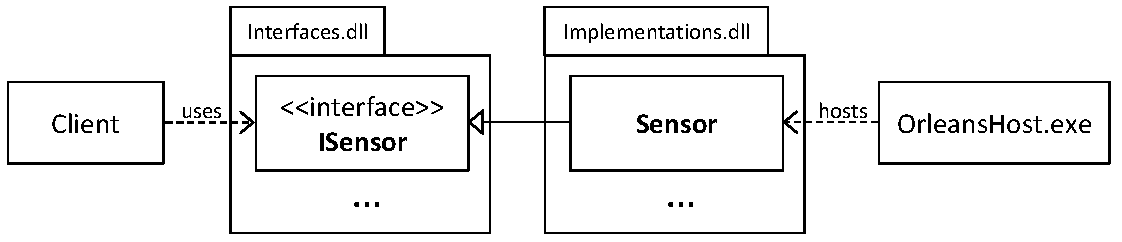
\includegraphics[width=\columnwidth]{orleans-hosting.pdf}%
\caption{Architektur von Anwendungen in Orleans}%
\label{fig:orleans-arch}%
\end{figure}

\subsubsection{Verwendung von Aktoren}

Der erste Schritt besteht darin, die Identität eines Aktors in eine Referenz umzuwandeln. Die Hilfsfunktion \lstinline{GetGrain} gibt als Resultat ein Stellvertreterobjekt für den angeforderten Aktor zurück, das die Schnittstelle des Aktors implementiert. Es ist nicht erforderlich, den Aktor explizit zu starten oder die tatsächliche physische Adresse herauszufinden. Diese Aufgaben sind Teil der Laufzeitumgebung von Orleans. In Programm~\ref{prog:orleans-actor-client} ist die Kommunikation mit einem Aktor dargestellt.

\begin{program}[!hbt]
\caption{Verwendung eines Aktors in Orleans}
\label{prog:orleans-actor-client}
\begin{CsCode}
var sensorId = Guid.Parse("eeb48102-c52f-4929-b7b3-da7cce96503f");
var sensor = GrainClient.GrainFactory.GetGrain<ISensor>(sensorId);
for(var i = 0; i < 10; i++)
  await sensor.AddMeasure(random.NextDouble());
Console.WriteLine($"Avg: {/+\textcolor{keywordColor}{await} sensor.GetAverage()+/}");
\end{CsCode}
\end{program}

%the dollar sign in the code above breaks the texniccenter syntax coloring. This invisible dollar escapes from math mode
\iffalse $ \fi

Das vom Klienten verwendete Stellvertreterobjekt ist automatisch von Orleans generiert. Standardmäßig wird der Stellvertreter schon zur Übersetzungszeit erstellt und als Teil der Schnittstellen"=Bibliothek ausgeliefert. Alternativ kann der Stellvertreter auch zur Laufzeit erzeugt werden.

\subsection{Persistente Aktoren}

Wenn der Zustand eines Aktors nur in Form von Klasseneigenschaften gespeichert ist, wie in Programm~\ref{prog:orleans-actor-impl} gezeigt, so ist dieser nur für die Dauer einer Aktivierung persistent. Sobald der Aktor wegen längerer Inaktivität deaktiviert wird, oder es zu einem Absturz kommt, geht der Zustand verloren. Für manche Daten, vor allem jene die sehr leicht zu berechnen sind, kann diese Form der Speicherung ausreichend sein. Häufig ist es aber von Vorteil, den Zustand eines Aktors dauerhaft zu persistieren. Man kann natürlich den Zustand selbst in einen persistenten Datenspeicher sichern und immer wieder laden. Das ist aber nicht notwendig, denn Orleans enthält bereits eine Lösung für diese immer wiederkehrende Anforderung. Um den Zustand eines Aktors zu persistieren, sind folgende Schritte erforderlich:

\begin{enumerate}
	\item Der Aktor muss von der Klasse \lstinline{Grain<T>} abgeleitet sein, wobei der Typ\-parameter \lstinline{T} ein Platzhalter für den tatsächlichen Typ des Zustandes ist. Dieser kann entweder ein primitiver Typ sein, oder eine beliebige Klasse.
	\item In der Konfiguration des Aktorsystems muss ein entsprechender Speichermechanismus registriert sein. Es gibt verschiedene bestehende Implementierungen, wie \zB Azure Table Storage oder SQL"=Datenbanken. Es ist auch möglich eigene Implementierungen zu verwenden.
	\item Außerdem ist es erforderlich die Klasse des Aktors mit dem Attribut \lstinline{StorageProvider} zu annotieren. Dieses Attribut stellt die Verbindung zu dem in Schritt zwei konfigurierten Speichermechanismus her.
\end{enumerate}

\begin{program}[!hbt]
\caption{Implementierung eines persistenten Aktors in Orleans}
\label{prog:orleans-persistent-actor}
\begin{CsCode}
[StorageProvider(ProviderName="<provider-name>")]
public class PersistentCounter : Grain<int>, IPersistentCounter   {
	public async Task<int> GetCount() => State;
	public async Task Increment() {
		State++;
		await WriteStateAsync();
	}
}
\end{CsCode}
\end{program}

In Programm~\ref{prog:orleans-persistent-actor} ist ein Aktor gezeigt, der seinen Zustand persistent speichert. In diesem Fall ist der Zustand in der Klasseneigenschaft \lstinline{State} lediglich eine natürliche Zahl. Änderungen werden erst nach einem Aufruf der Funktion \lstinline{WriteStateAsync} in den persistenten Speicher geschrieben. Ansonsten würde sich der Zustand nur für die aktuelle Aktivierung ändern. Bei jeder erneuten Aktivierung lädt Orleans den Zustand automatisch aus dem persistenten Speicher.

\subsection{Cluster}

Ein Cluster besteht aus einer Menge von Silos, die zu einer Einheit verbunden sind. Meistens läuft nur eine Silo auf einem Rechner. Es sind aber auch mehrere möglich. Jeder Silo muss wissen, welche anderen Silos ebenfalls Mitglieder des Clusters sind. Die Anzahl der Silos bestimmt nämlich, wie der  Wertebereich der Identität der Aktoren auf die Silos aufgeteilt ist. Sie müssen sozusagen einen Konsens über die Liste von Mitgliedern finden, damit alle von einer global einheitlichen Sichtweise ausgehen. Eine Lösung für diese in verteilten Systemen häufig auftretende Problemstellung, ist die Verwendung des Paxos"=Algorithmus~\cite{Lamport:1998:PP:279227.279229}. Eine Einschränkung dieses Algorithmus ist jedoch, dass Entscheidungsfindung eine Mehrheit der Mitglieder, ein sogenanntes Quorum, erfordert. Orleans hingegen setzt auf ein eigens entwickeltes Protokoll, das die Liste der Mitglieder in einer externen tabellenartige Datenstruktur speichert. Dieses Protokoll ist nicht auf eine Mehrheitsentscheidung angewiesen.

In der Mitgliederliste hat jeder Silo einen eigenen Eintrag, der \zB die Information enthält, ob dieser online oder offline ist. Diese Datenstruktur erfüllt zwei wichtige Aufgaben. Erstens können damit Silos die Liste der übrigen funktionstüchtigen Teilnehmer ermitteln. Zweitens benötigen auch Klienten diese Liste, damit sie mit Silos in Kontakt treten können. Nachfolgend ist erläutert, wie die Mitglieder eines Clusters ermittelt werden~\cite{Bernstein2014}:

\begin{itemize}
	\item Jeder Silo trägt sich nach dem Starten in die Mitgliederliste ein.
	\item Die Silos im Cluster überwachen sich gegenseitig durch das periodische Senden von Kontrollnachrichten. Die Identität jedes Aktors wird mit Hilfe eines konsistenten Hashverfahren auf einen zyklischen Wertebereich abgebildet. Damit sind die Silos geordnet und jeder kann eine gewisse Anzahl von zu überwachenden Nachfolgern auswählen.
	\item Wenn mehrere Kontrollnachrichten von Silo $S$ an Silo $T$ fehlschlagen, vermerkt $S$ diesen Vorfall in der Mitgliederliste bei $T$.
	\item Übersteigt die Anzahl von verdächtigen Vorfällen innerhalb einer gewissen Periode einen Grenzwert, so deklariert Silo $S$ Silo $T$ als nicht mehr verfügbar. Anschließend sendet $S$ eine Aufforderung an alle, die Mitgliederliste neu zu laden. Wenn alle Silos ihre Mitgliederliste aktualisiert haben, ist Silo $T$ nicht mehr Teil des Clusters.
\end{itemize}

Die Konfiguration eines Clusters ist durch das dynamische Mitgliederprotokoll in Orleans sehr einfach. Ein Silo benötigt einen TCP"=Port für die Kommunikation mit anderen Silos und einen weiteren für die Verbindung zu Klienten. Sowohl bei allen Silos als auch bei den Klienten muss der selbe Speicher für die externe Mitgliederliste definiert sein. Wenn alle Einstellungen korrekt konfiguriert sind, können neue Silos einfach zur Laufzeit hinzugefügt oder entfernt werden.

\subsection{Lastverteilung in einem Cluster}

Verwender von Orleans haben nur begrenzten Einfluss auf die Verteilung der Aktivierungen von Aktoren auf die Silos eines Clusters. Ein Grundgedanke von Orleans, ist es derartige Entscheidungen in der Laufzeitumgebung zu treffen und somit den Verwender zu entlasten. Anstelle Aktoren direkt mit einem deterministischen Verfahren Silos zuzuordnen, speichert Orleans den Ort einer Aktivierung in einem auf allen Silos verteilten Verzeichnis~\cite[5]{virtualActors}. Durch diese zusätzliche Indirektion hat die Laufzeitumgebung von Orleans mehr Freiheiten, die Aktoren zu platzieren und dynamisch umzuverteilen. Wenn ein Klient mit einem Aktor interagieren will, sind dafür zwei Schritte notwendig. Er sendet seine Anfrage an einen beliebigen Silo im Cluster. Dieser muss zuerst den Silo auffinden, der für die Partition des verteilten Verzeichnisses für den angeforderten Aktor zuständig ist. Dort befindet sich die Information, auf welchem Silo möglicherweise bereits eine Aktivierung läuft. Wenn noch keine Aktivierung existiert, muss diese erst erzeugt werden. Der zweite Schritt bestehen darin, den Klienten auf den Silo der tatsächlichen Aktivierung weiterzuleiten.

Das Verzeichnis ist als eine verteilte Hashtabelle implementiert, in der jeder Knoten für einen anderen Teil des gesamten Wertebereichs verantwortlich ist~\cite{Stoica:2001:CSP:383059.383071}. Sowohl die Identität eines Aktors als auch die Identität eines Silos werden mit Hilfe eines konsistenten Hashverfahrens auf den selben zirkulären Wertebereich abgebildet. Durch die Gleichverteilung der Hashfunktion ergibt sich automatisch eine gleichmäßige Verteilung der Identitäten der Aktoren auf alle Silos eines Clusters. Der Vorteil dieses Verfahrens gegenüber klassischer Hashverfahren liegt darin, dass sich bei einer Änderung in der Mitgliederliste im Durchschnitt die Zuordnung von nur $K/n$ Aktoren ändert, wobei $K$ die Größe des Wertebereichs ist und $n$ die Anzahl der Silos. Bei der Zuweisung mit einem normalen Hashverfahren würde sich praktisch die gesamte Zuordnung ändern.

Ein Eintrag in dem verteilten Verzeichnis beinhaltet die Identität des Aktors und die Adresse des Silos, auf dem eine Aktivierung eines Aktor bereits existiert. Wenn noch keine Aktivierung existiert, muss eine neue Aktivierung zuerst erzeugt werden. Standardmäßig wird eine Aktivierung auf einem zufällig ausgewählten Silo gestartet. Es gibt aber auch noch weitere Strategien, wie \zB die Lastverteilung aufgrund der Anzahl von Aktivierungen. In Abbildung~\ref{fig:orleans-acor-placement} ist noch einmal dargestellt, wie das verteilte Verzeichnis funktioniert.

\begin{figure}[!hbt]%
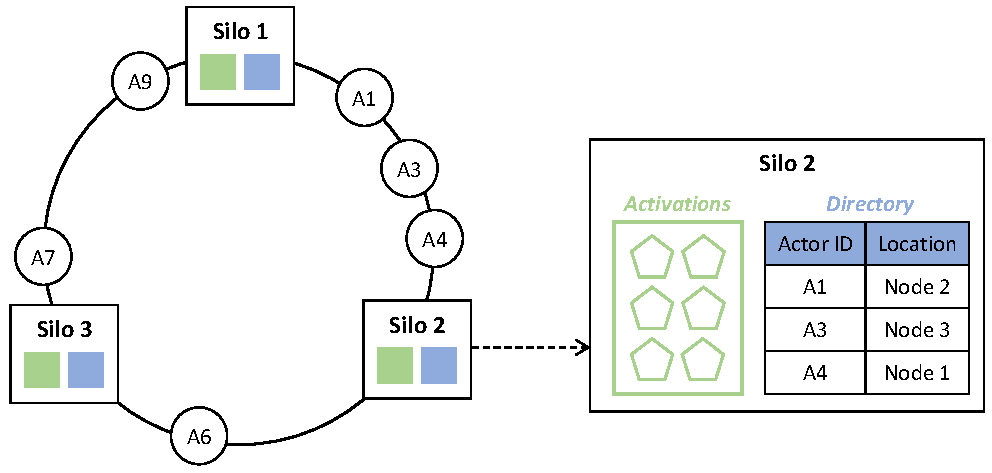
\includegraphics[width=\columnwidth]{orleans-actor-placement.pdf}%
\caption{Bla}%
\label{fig:orleans-acor-placement}%
\end{figure}

Die zusätzliche Indirektion durch das verteilte Verzeichnis macht das Auffinden des Ortes einer Aktivierung zu einer aufwändigen Operation. Aus diesem Grund vermerkt jeder Silo erfolgreich aufgelöste Anfragen in einem lokalen Zwischenspeicher.

\subsection{Fehlerbehandlung}

Ein Aspekt in dem Orleans wesentlich vom traditionellen Aktorenmodell abweicht, ist die Behandlung von Fehlern. Wie der Abschnitt über Erlang gezeigt hat, ist eine Konsequenz des asynchronen Nachrichtenaustauschs, dass Fehler nicht vom Aufrufer behandelt werden können. Stattdessen muss jemand anderer, den an einem möglicherweise entfernten Ort aufgetretenen Fehler behandeln. Dazu ist im Supervisorbaum festgelegt, welche Aktoren sich um die Fehler von anderen Aktoren kümmern. Der Supervisor bekommt eine Fehlernachricht und muss über das weitere Vorgehen entscheiden.

Mit dem Programmiermodell von Orleans ist es dem Aufrufer möglich, Fehler selbst zu behandeln. Tritt ein Fehler bei einem Funktionsaufruf auf, wird dieser zum Klienten gesendet und dort wieder als gewöhnliche .NET"=Ausnahme geworfen. Die dafür benötigte Logik ist in den von Orleans automatisch generierten Stellvertreterobjekten implementiert. Es ist nicht notwendig, Aktoren neu zu starten, weil sie ohnehin beim nächsten Aufruf automatisch neu gestartet werden.

Standardmäßig wird in Orleans eine Nachricht höchstens einmal zugestellt. Der Aufrufer einer Methode bekommt entweder im Erfolgsfall ein Ergebnis zurück, oder wenn die Nachricht verloren ging, eine Zeitüberschreitung, die sich als .NET"=Ausnahme manifestiert. Im Fehlerfall ist der Anwender selbst verantwortlich, die Anfrage zu wiederholen. Alternativ kann auch eine automatische Wiederholung von nicht beantworteten Anfragen eingestellt werden. Das kann aber zu einer mehrfachen Zustellung der selben Nachricht führen. In diesem Fall müssen die aufgerufenen Methoden idempotent sein oder selbst eine Duplikaterkennung durchführen.

Es ist normalerweise garantiert, dass nur eine Aktivierung eines Aktors zur selben Zeit existiert. Es gibt aber einen Ausnahmefall in dem diese Garantie nicht gilt. Wenn nach einem Ausfall eines Silos zwei Silos noch nicht die selbe Sichtweise auf die Mitgliederliste haben, kann es sein, dass beide die Aktivierung eines Aktors anfordern. In diesem Fall existieren zwei Aktivierungen des selben Aktors gleichzeitig. Sobald die Silos die selbe Sichtweise auf die Mitgliederliste haben, wird eine der Aktivierungen terminiert, sodass schlussendlich nur noch eine übrig bleibt. Diese Art der Konsistenz wird als \textit{Eventual Consistency} bezeichnet, weil schlussendlich ein konsistenter Zustand erreicht wird. In Orleans wird also die Verfügbarkeit der Konsistenz vorgezogen. Bei persistenten Aktoren kann das beschriebene Phänomen leicht zu unerwarteten Inkonsistenzen führen. Wenn beide Aktivierungen den selben Zustand aus dem externen Speicher laden und wieder speichern, geht eine der beiden Änderungen verloren.

\section{Aktorenmodell und Microservices}

Bis hier her ist es möglicherweise nicht ganz offensichtlich, wie das Aktorenmodell zu den anderen in dieser Arbeit behandelten Themen in Verbindung steht. Daher ist das Ziel dieses Abschnitts, verschiedene mögliche Sichtweisen auf die Beziehung zwischen dem Aktorenmodell und der Microservice"=Architektur darzustellen.

Zuerst ist es aber hilfreich, die Gemeinsamkeiten zwischen diesen beiden Ansätzen herauszuarbeiten. Zunächst handelt es sich bei beiden um ein verteiltes System für die Realisierung von möglichst skalierbaren und robusten Anwendungen. Sie haben ebenfalls beide ein Konzept, Software in abgeschlossene Komponenten zu zerlegen. In der Microservice"=Architektur sind das Dienste und im Aktorenmodell Aktoren. Ein Ziel dieser Zerlegung ist, die Verantwortlichkeiten der Anwendung besser zu trennen, damit die Abhängigkeit zwischen Komponenten gering ist. Ohne eine saubere Trennung entsteht eine stark verwobene Architektur, bei der jede Änderung nicht vorhersehbare Auswirkungen auf den Rest des Systems bedeutet. 

Beide Ansätze zeichnen sich durch gute Skalierbarkeit aus. Sie setzen auf eigenständige Komponenten, die nur per Nachrichtenaustausch miteinander interagieren. Dadurch können sie sehr leicht auf mehrere Rechner verteilt werden. Es gibt bestimmt noch weitere Gemeinsamkeiten, aber die gerade beschriebenen sind sicherlich eine der größten. 

In Abschnitt~\ref{subsubsec:microservices-disadvantages} wurde bereits erläutert, dass viele Experten davon abraten, neue Anwendungen mit einer Microservice"=Architektur zu beginnen. Dafür ist nämlich ein großes Domänenwissen notwendig, das am Anfang noch nicht vorhanden ist. Daher kann es von Vorteil sein, neue Projekte zuerst auf Basis des Aktorenmodells zu beginnen und erst bei Bedarf eigenständige Dienste herauszulösen. Dieses als evolutionäre Architektur bekannte Vorgehen ist im Bereich von Microservices gängige Praxis. 

Bei vielen Microservices fällt die Wahl für ein Kommunikationsprotokoll auf eine Kombination aus HTTP und REST. Es mag aber durchaus Gründe für eine andere Wahl geben. Mit Aktoren ist es nicht notwendig, ein Kommunikationsprotokoll festzulegen. Die Kommunikationsfähigkeit von Aktoren ist eine inhärente Eigenschaft des Aktorenmodells. Es ist sogar naheliegend, dass die für Aktoren eingesetzten binären Protokolle effizienter sind als HTTP und REST.

Wenn man einen Aktor als Service -- oder eher als Nanoservice -- bezeichnet, könnte man das Aktorenmodell als Implementierung der Microservice"=Architektur sehen. Ein Aktor erfüllt nämlich alle in Abschnitt~\ref{sec:ms-characteristics} beschriebenen Charakteristiken eines Microservices. Beginnend bei der Modularisierung, über die Größe, den Nachrichtenaustausch bis hin zu flexiblen Möglichkeiten, Aktoren auszurollen. Genau so gut kann das Aktorenmodell ein möglicher Bestandteil der Microservice"=Architektur sein, in der es nur für vereinzelte Dienste zum Einsatz kommt. Diese Interpretationen erfordern aber eine großzügige Auslegung, weil beide Konzepte für einen objektiven Vergleich zu unterschiedlich sind. Ein mathematisches Modell und eine serviceorientierten Architektur sind schwer vergleichbar.

\section{Zusammenfassung}

In diesem Kapitel wurde das Aktorenmodell, hauptsächlich anhand von \mbox{Erlang} und Orleans, ausführlich erläutert. Ein Aktor ist eine fundamentale Recheneinheit, die Befehle ausführt, Daten speichert und mit anderen Aktoren kommuniziert. In Erlang wurde ein Aktor als \textit{Prozess} und in Orleans als \textit{Grain} bezeichnet. Es ist aber in beiden Fällen dasselbe Konzept.

Erlang ist eine funktionale Programmiersprache, mit einem Prozessmodell, das dem Aktorenmodell entspricht. Jeder Prozess ist eine leichtgewichtige und eigenständige Berechnungseinheit, die nur per asynchrone Nachrichten mit anderen Prozessen kommuniziert. Dieses Programmiermodell fördert die Skalierbarkeit, weil Prozesse auf beliebig viele Rechner verteilbar sind. Außerdem ist es sehr robust, weil sich ein Fehler nur auf einen Prozess auswirkt. Es ist aber notwendig, dass sich Prozesse gegenseitig überwachen und im Fehlerfall entsprechende Handlungen setzen. In vielen Fällen ist diese Behandlung einfach ein Neustart des fehlgeschlagenen Prozesses.

Mit dem auf der .NET"=Plattform entwickelten Framework Orleans wurde versucht, das Aktorenmodell zu vereinfachen. Dazu hat man viele Entscheidungen, die normalerweise ein Programmierer während der Entwicklung eines verteilten Systems trifft, bereits in der Laufzeitumgebung von Orleans festgelegt. Das Programmiermodell von Orleans hat viele Gemeinsamkeiten mit der objektorientierten Programmierung. Es ist aber von Grund auf für verteilte Systeme konzipiert. Dieses stark vereinfachte Programmiermodell versucht, die Produktivität der Entwickler zu maximieren. Der Preis dafür ist aber eine geringere Flexibilität als beispielsweise bei Erlang.